%\documentclass[english, times, mirror]{revdetua}
% use this if you're writing in portuguese:
\documentclass[portuguese, times, mirror]{revdetua}

\usepackage[utf8]{inputenc}
\usepackage{graphicx}
\usepackage{hyperref}

\usepackage{amsmath}
\usepackage{mathtools}

\usepackage{caption}
\usepackage{listings}
\usepackage{color}

\definecolor{dkgreen}{rgb}{0,0.6,0}
\definecolor{gray}{rgb}{0.5,0.5,0.5}
\definecolor{mauve}{rgb}{0.58,0,0.82}

\lstset{frame=tb,
  language=Java,    
  aboveskip=3mm,
  belowskip=3mm,
  showstringspaces=false,
  columns=flexible,
  basicstyle={\small\ttfamily},
  numbers=none,
  numberstyle=\tiny\color{gray},
  keywordstyle=\color{blue},
  commentstyle=\color{dkgreen},
  stringstyle=\color{mauve},
  breaklines=true,
  breakatwhitespace=true,
  tabsize=3
}

\usepackage{tikz}
\usepackage{pgfplots}

% correct bad hyphenation here
\hyphenation{op-tical net-works semi-conduc-tor}

\begin{document}

\Header{1}{1}{Outubro}{2016}{1}
% Note: the month must be in Portuguese

\title{Visão por Computador 2016-17, Guia Prático N.º 3}
\author{Rui Oliveira, Tomás Rodrigues\\ DETI, Universidade de Aveiro \\ Aveiro, Portugal \\ \{ruipedrooliveira, tomasrodrigues\}@ua.pt}
% you should be able to use the \and keyword, but the deti format doesn't like it, for some reason
\maketitle

\begin{resumo}


Pretende-se através deste relatório expor sob forma escrita, o nosso desempenho e objetivos alcançados na aula prática n.3 da unidade curricular de Visão por Computador do Mestrado Integrado de Engenharia de Computadores e Telemática.

Neste relatório pretenderemos explicar as soluções por nós encontradas para a resolução dos diferentes problemas propostos.


\end{resumo} 

\begin{palavraschave} %
visão, computador, imagem digital, opencv, c++, 
 \end{palavraschave} %




\section{Repositório: código fonte}


Todas as soluções dos problemas propostos estão disponível através do seguinte repositório (gitHub) criado para o efeito. \\

\href{http://github.com/toomyy94/CV1617-68779-68129}{http://github.com/toomyy94/CV1617-68779-68129}
\\


A resolução dos problemas do presente guia encontram-se na pasta aula3. 



\section{Problemas propostos}



\subsection{Problema \#1}

\subsubsection{Enunciado}
\textit{ Implement a program to capture images from your digital camera (VideoCapture class) and
include the capability of showing the grayscale and the black and white version of the acquired
image.
Use all the functionalities of the OpenCv library, namely the use of the functions cvtColor and
adaptiveThreshold.}


\subsubsection{Resolução e principais conclusões}


Inicialmente começámos por converter para escala de cinzento (\texttt{CV\_BGR2GRAY}) a imagem obtida através da class \texttt{VideoCapture}. Posteriormente utilizá-mos o método \texttt{adaptiveThreshold} com os argumentos escolhidos pelo utilizador. Este método apenas pode ser aplicado a imagens com um único canal de 8 bits, daí a conversão para escala de cinza. 

Mais especificações sobre a função \texttt{adaptiveThreshold} e os seus argumentos podem ser consultados no \href{http://docs.opencv.org/2.4/modules/imgproc/doc/miscellaneous_transformations.html}{manual online do OpenCV}. 



%Fazemos a captura de vídeo da camara através da VideoCapture class e posteriormente fazemos a conversão de cada frame para uma imagem de 8bits com a função cvtColor para psoteriormente podermos aplicar então o adaptativeThreshold


\newpage

A imagem seguinte demonstra a interação com o utilizador que é permitida. 

\begin{figure}[ht!]
\centering
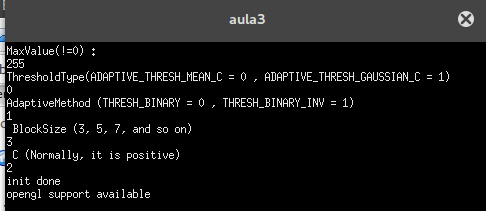
\includegraphics[width=70mm]{img/ex1_2.png}
\caption{Interação com o utilizador}
\end{figure}


À esquerda encontra-se o resultado proveniente da conversão para escala de cinzento (\texttt{CV\_BGR2GRAY}) e à direita a aplicação da função \texttt{adaptiveThreshold} com os parametros introduzidos pelo utilizador. 

\begin{figure}[ht!]
\centering
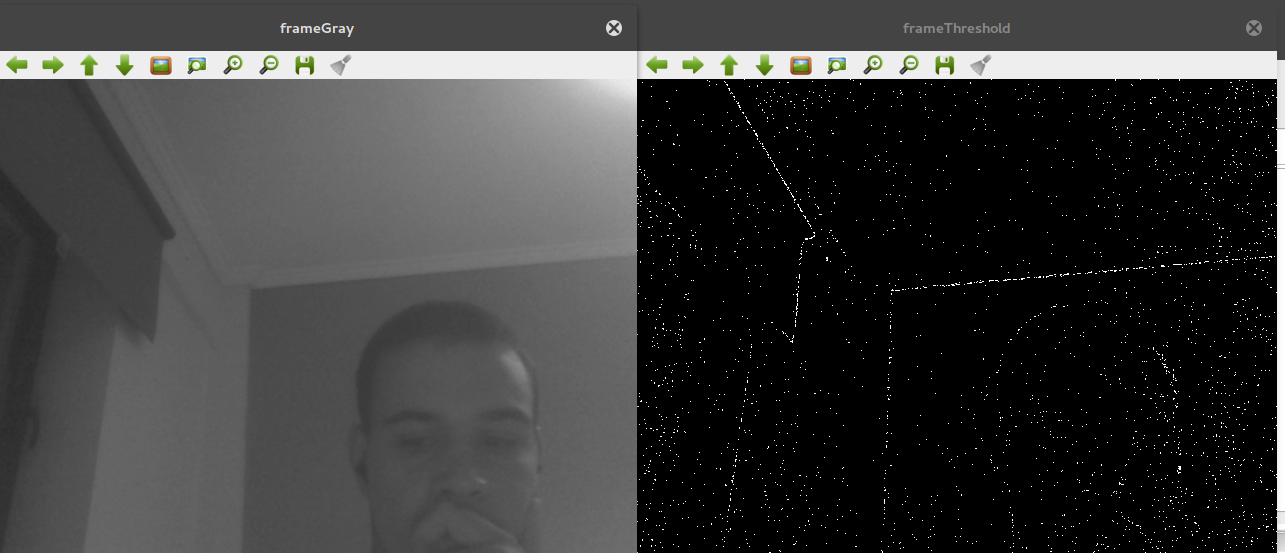
\includegraphics[width=70mm]{img/ex1_!.png}
\caption{Resultado obtido}
\end{figure}





\begin{figure}[ht!]
\centering
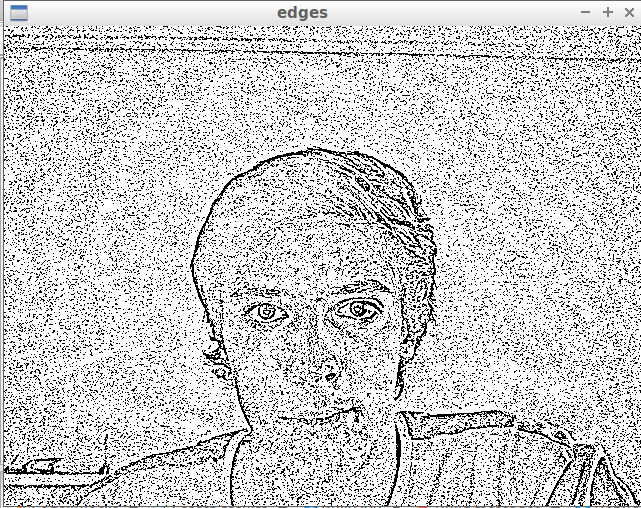
\includegraphics[width=70mm]{img/ex1.png}
\caption{Resultado após execução do problema 1.}
\end{figure}

\subsection{Problema \#2}

\subsubsection{Enunciado}
\textit{ Include an option in the previous program to explore the use of the threshold function to obtain
also a binary image.}

\subsubsection{Resolução e principais conclusões}



Durante a recolha de imagem é possivel aplicar os seguintes thresholding, através a introdução dos seguintes caracteres pelo teclado. 

\begin{itemize}
\item 0: Binary
\item 1: Binary Inverted
\item 2: Threshold Truncated
\item 3: Threshold to Zero
\item 4: Threshold to Zero Inverted
\item q: Exit
\end{itemize}



\begin{figure}[ht!]
\centering
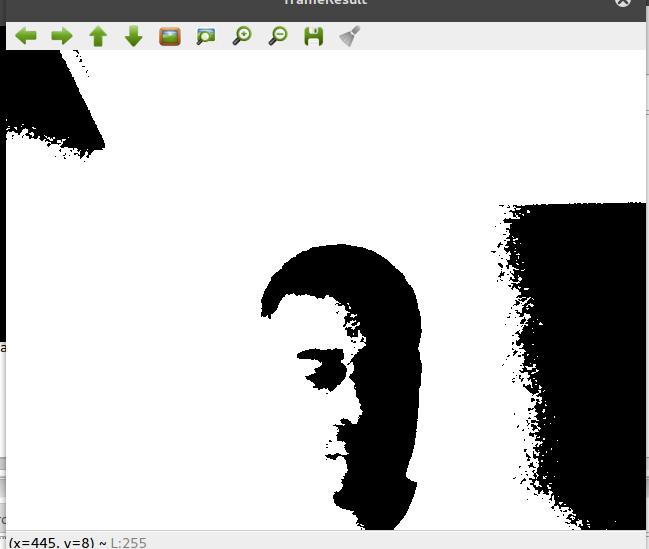
\includegraphics[width=70mm]{img/2_1.png}
\caption{Binary}
\end{figure}

\begin{figure}[ht!]
\centering
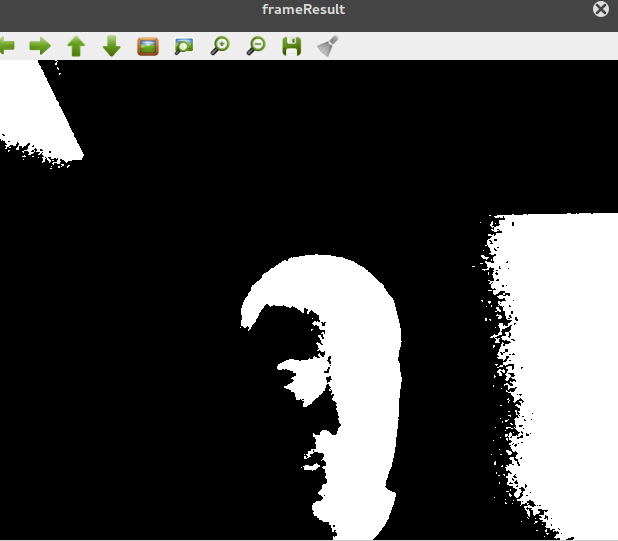
\includegraphics[width=70mm]{img/2_2.png}
\caption{Binary Inverted}
\end{figure}

\begin{figure}[ht!]
\centering
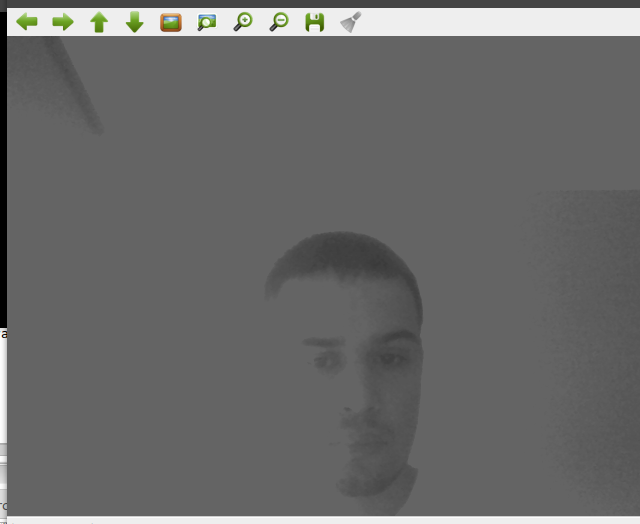
\includegraphics[width=70mm]{img/2_3.png}
\caption{Threshold Truncated}
\end{figure}

\begin{figure}[ht!]
\centering
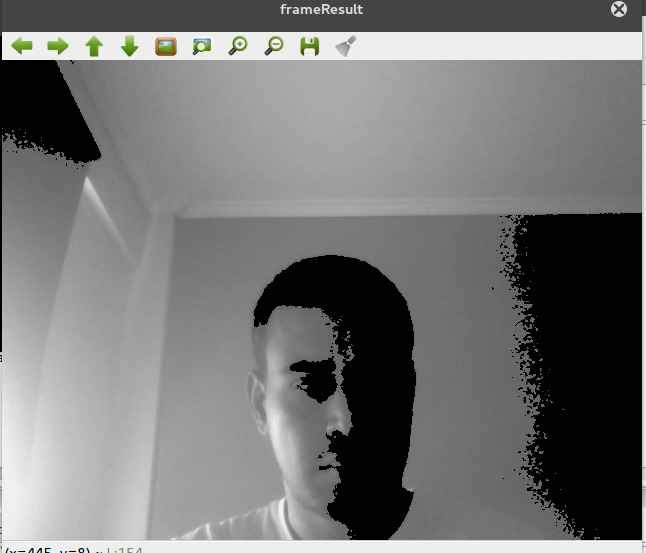
\includegraphics[width=70mm]{img/2_4.png}
\caption{Threshold to Zero}
\end{figure}

\begin{figure}[ht!]
\centering
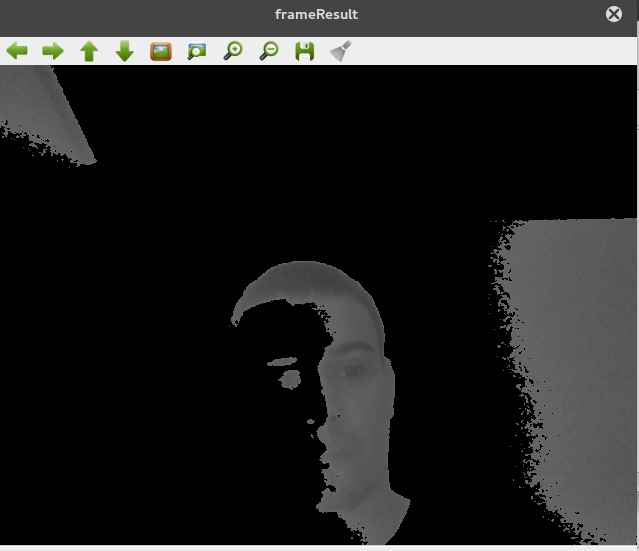
\includegraphics[width=70mm]{img/2_5.png}
\caption{Threshold to Zero Inverted}
\end{figure}

%%%%%%%%%%%%%%%%%%%%%%%%%%%%%%%%%






\newpage

\subsection{Problema \#3}

\subsubsection{Enunciado}
\textit{ Implement a program to perform a simple skin color detector based on chromaticity or other color
properties.}

\subsubsection{Resolução e principais conclusões}

Neste exercício tentámos obter um realce da pele humana atravéz essencialmente do contorno. Este abordagem não nos deu idealmente o que pretendíamos, falhando a detenção da pele em alguns aspetos como se pode ver na imagem abaixo.


\begin{figure}[ht!]
\centering
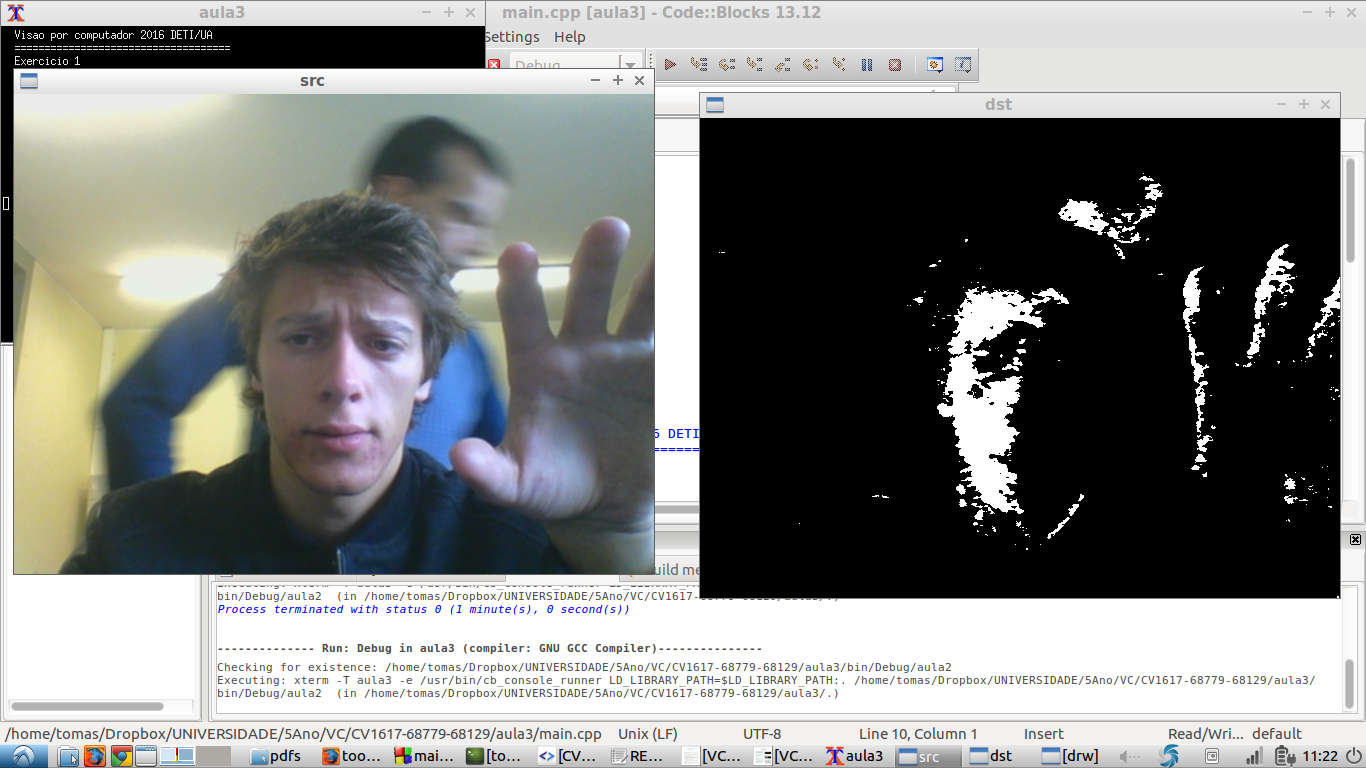
\includegraphics[width=70mm]{img/ex3.png}
\caption{Resultado após execução do problema 3.}
\end{figure}

%%%%%%%%%%%%%%%%%%%%%%%%
\subsection{Problema \#4}

\subsubsection{Enunciado}
\textit{ Implement a program to capture images from your digital camera and explore the use of filters
to modify the images acquired.}

\subsubsection{Resolução e principais conclusões}

Para este problema usámos duas funções de média que o opencv disponibiliza, a medianBlur e a gaussianBlur. Como era esperado verificámos que há medida que aumentávamos o tamanho do ksize a imagem ia ficando mais desfocada/smoth. Estas funções podem ser usadas para atenuar possível ruído em imagens!
    

\texttt{medianBlur ( frame, frameResult, 15 );}

\begin{figure}[ht!]
\centering
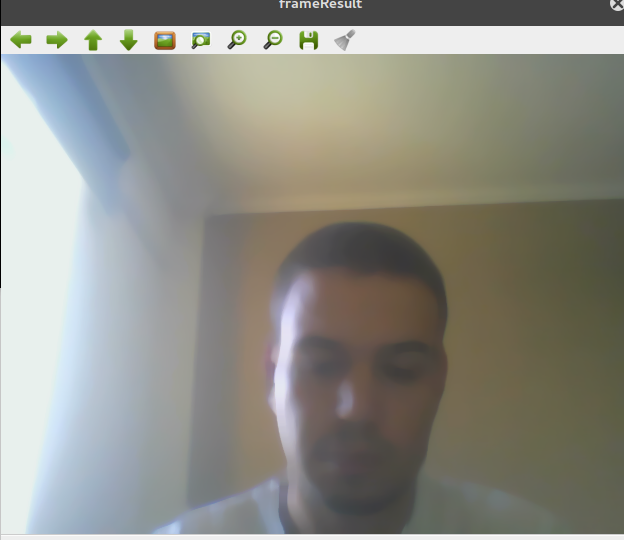
\includegraphics[width=70mm]{img/4_1.png}
\caption{medianBlur}
\end{figure}


\texttt{blur( frame, frameResult, Size( 10, 10 ), Point(-1,-1));}

\begin{figure}[ht!]
\centering
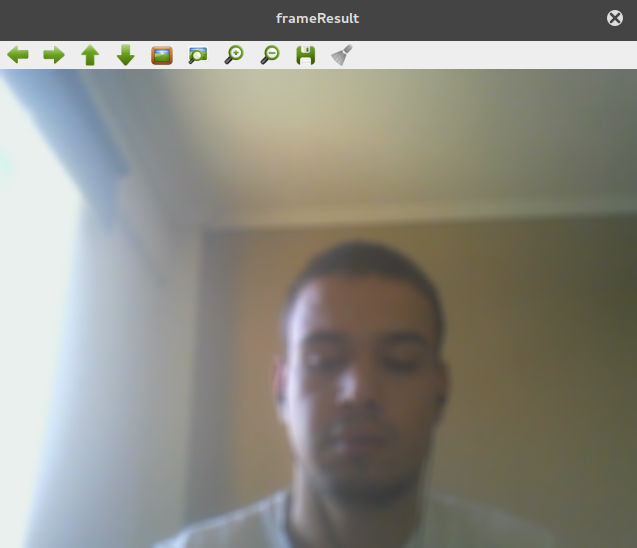
\includegraphics[width=70mm]{img/4_2.png}
\caption{blur}
\end{figure}

\newpage

%%%%%%%%%%%%%%%%%%%%%%%%
\subsection{Problema \#5}

\subsubsection{Enunciado}
\textit{Implement a program to capture images from your digital camera and calculate the histogram of
each one of the chan}

\subsubsection{Resolução e principais conclusões}

Depois de uma pequena pesquisa encontrámos uma solução ao problema que nos separa então a imagem em 3 componentes(R,G,B). Estabelecemos o número de barras do histograma em 256 e computámos e desenhámos o histograma nos 3 canais respetivos.


\begin{figure}[ht!]
\centering
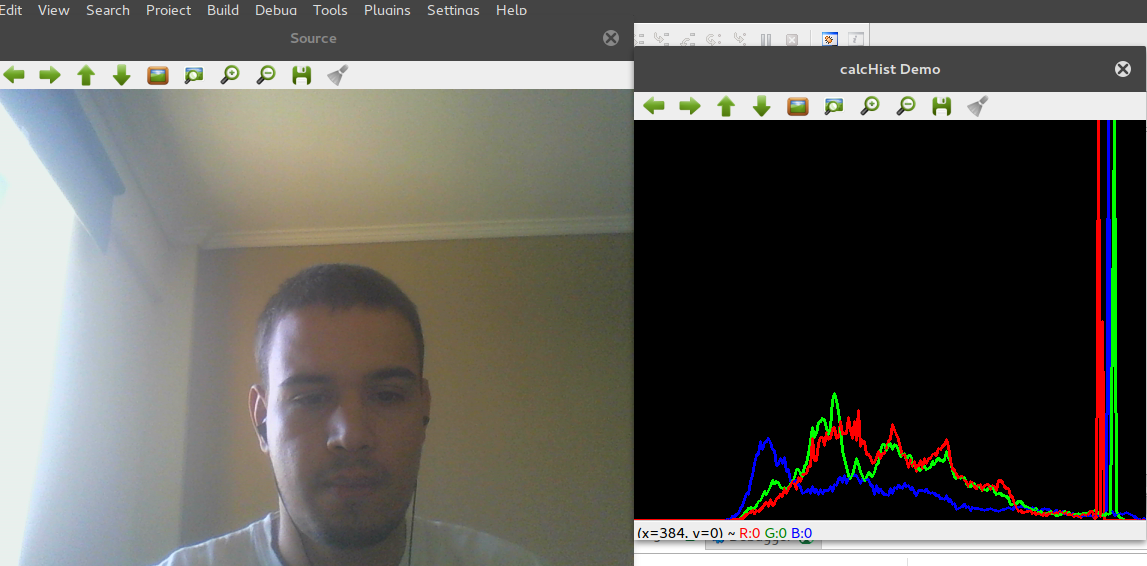
\includegraphics[width=70mm]{img/5_1.png}
\caption{Histograma da imagem obtida pela camara. 3 Canais. }
\end{figure}

\subsection{Problema \#6}

\subsubsection{Enunciado}
\textit{Include in the previous program the capability of apply histogram normalization. Visualize also
the new histogram(s) obtained and comment the results.}

\subsubsection{Resolução e principais conclusões}

Este problema foi resolvido com recurso á função do opencv já existente \textit{equalizeHist}. Resultados obtidos podem ser encontrados abaixo.

\begin{figure}[ht!]
\centering
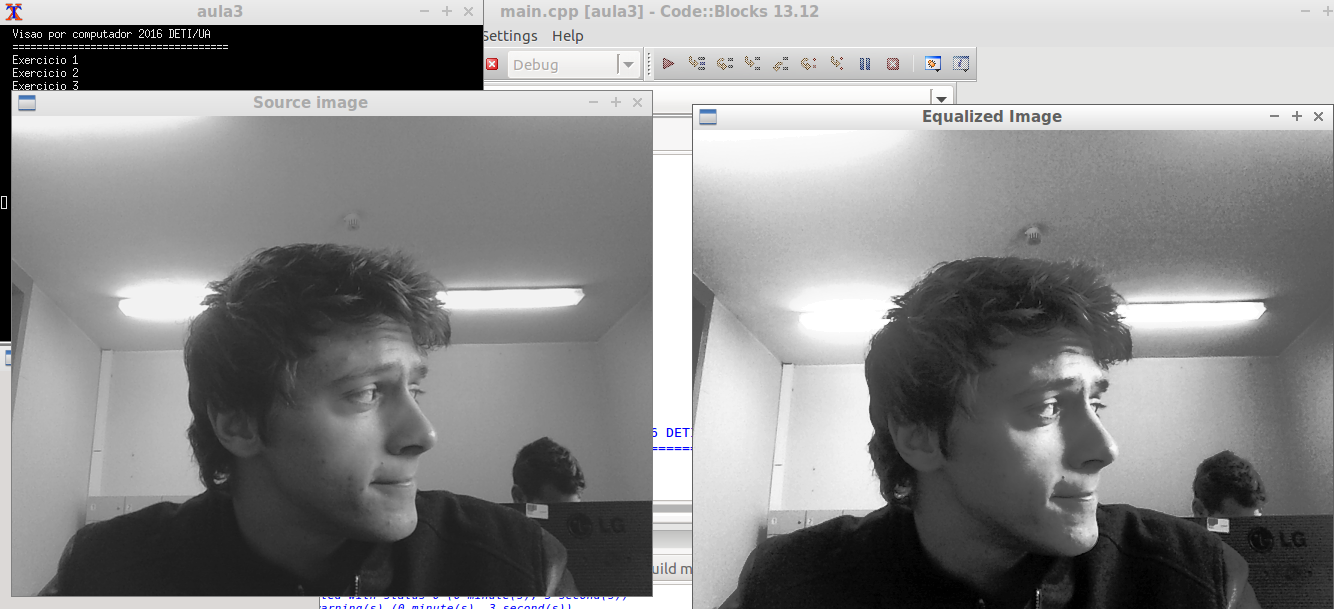
\includegraphics[width=80mm]{img/ex6.png}
\caption{Resultado após execução do problema 6.}
\end{figure}

\subsection{Problema \#7}

\subsubsection{Enunciado}
\textit{Implement a program that loads two images and compare the histograms of both.}

\subsubsection{Resolução e principais conclusões}



Concluímos que os histogramas obtidos para as duas imagens – imagem original e a sua inversa – são exatamente iguais, uma vez que a distribuição de cores presentes são exatamente as mesmas.  


\begin{figure}[ht!]
\centering
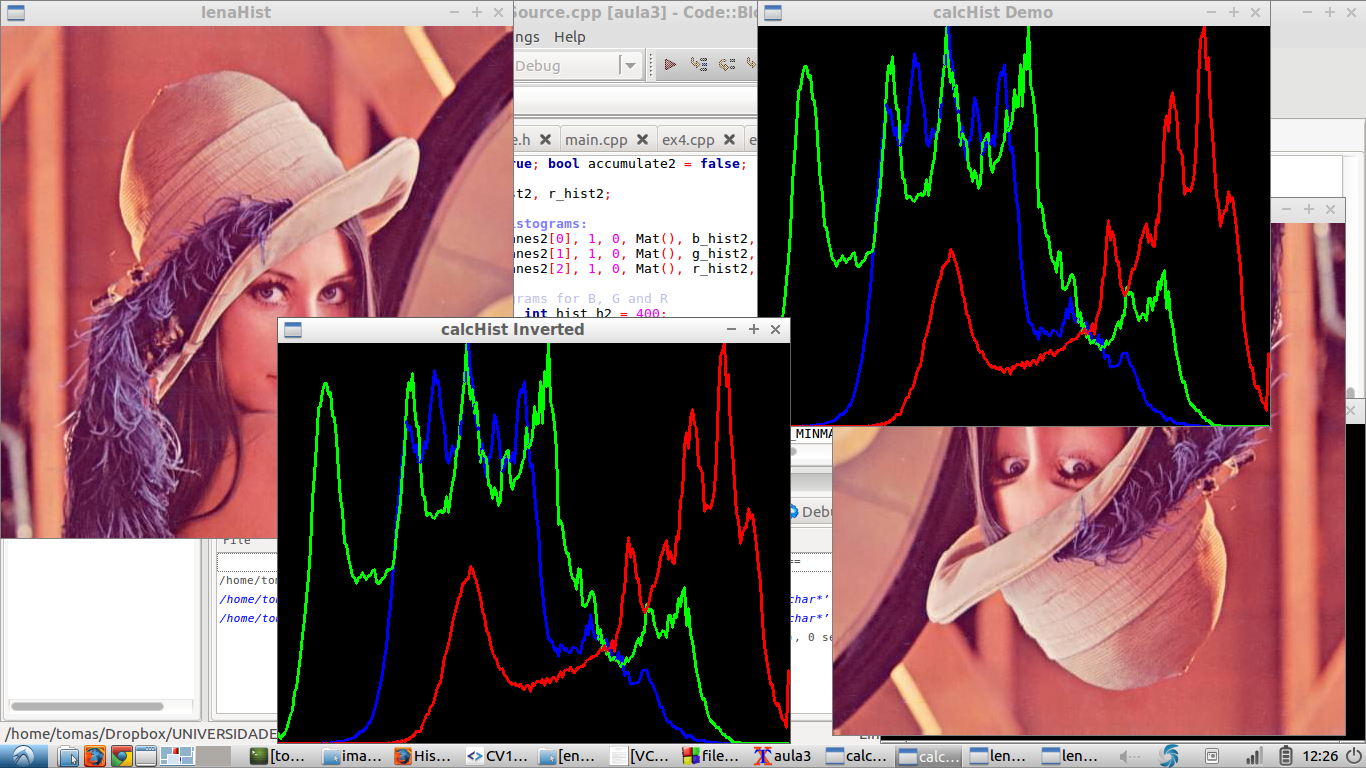
\includegraphics[width=80mm]{img/ex7.png}
\caption{Resultado após execução do problema 7.}
\end{figure}



\begin{thebibliography}{1} % 9



\bibitem{fsound}
Neves, A. J. R.; Dias, P. Slides teóricos Visão por Computador - Aula 2 (2016)


\bibitem{vtk}
OpenCV. \href{hhttp://docs.opencv.org/}{Opencv Documentation}. Web. 24 Outubro 2016. 




\end{thebibliography}

\end{document}
